\chapter{Methodology} \label{cp:methodology}

\section{Apparatus} \label{sec:apparatus}
A Schlieren Imaging System is set up to view flow through a converging-diverging nozzle in the test section of the supersonic wind tunnel. The wind tunnel is seen in \autoref{fig:supersonic_wind_tunnel} with the nozzle shown in \autoref{fig:de_laval_nozzle}. A light source is reflected off a concave mirror which passes the light through the test section. Then, the light is reflected by another concave mirror towards a whiteboard after some of the focused light is blocked by a razor's edge. A camera is used to capture the projection on the whiteboard (see \autoref{fig:schlieren_projection}) which is connected to a delay generator to match the images with pressure data from taps in the nozzle. The camera images and pressure transducer data are collected using data acquisition software on a computer. 

\begin{figure}[htpb]
    \centering
    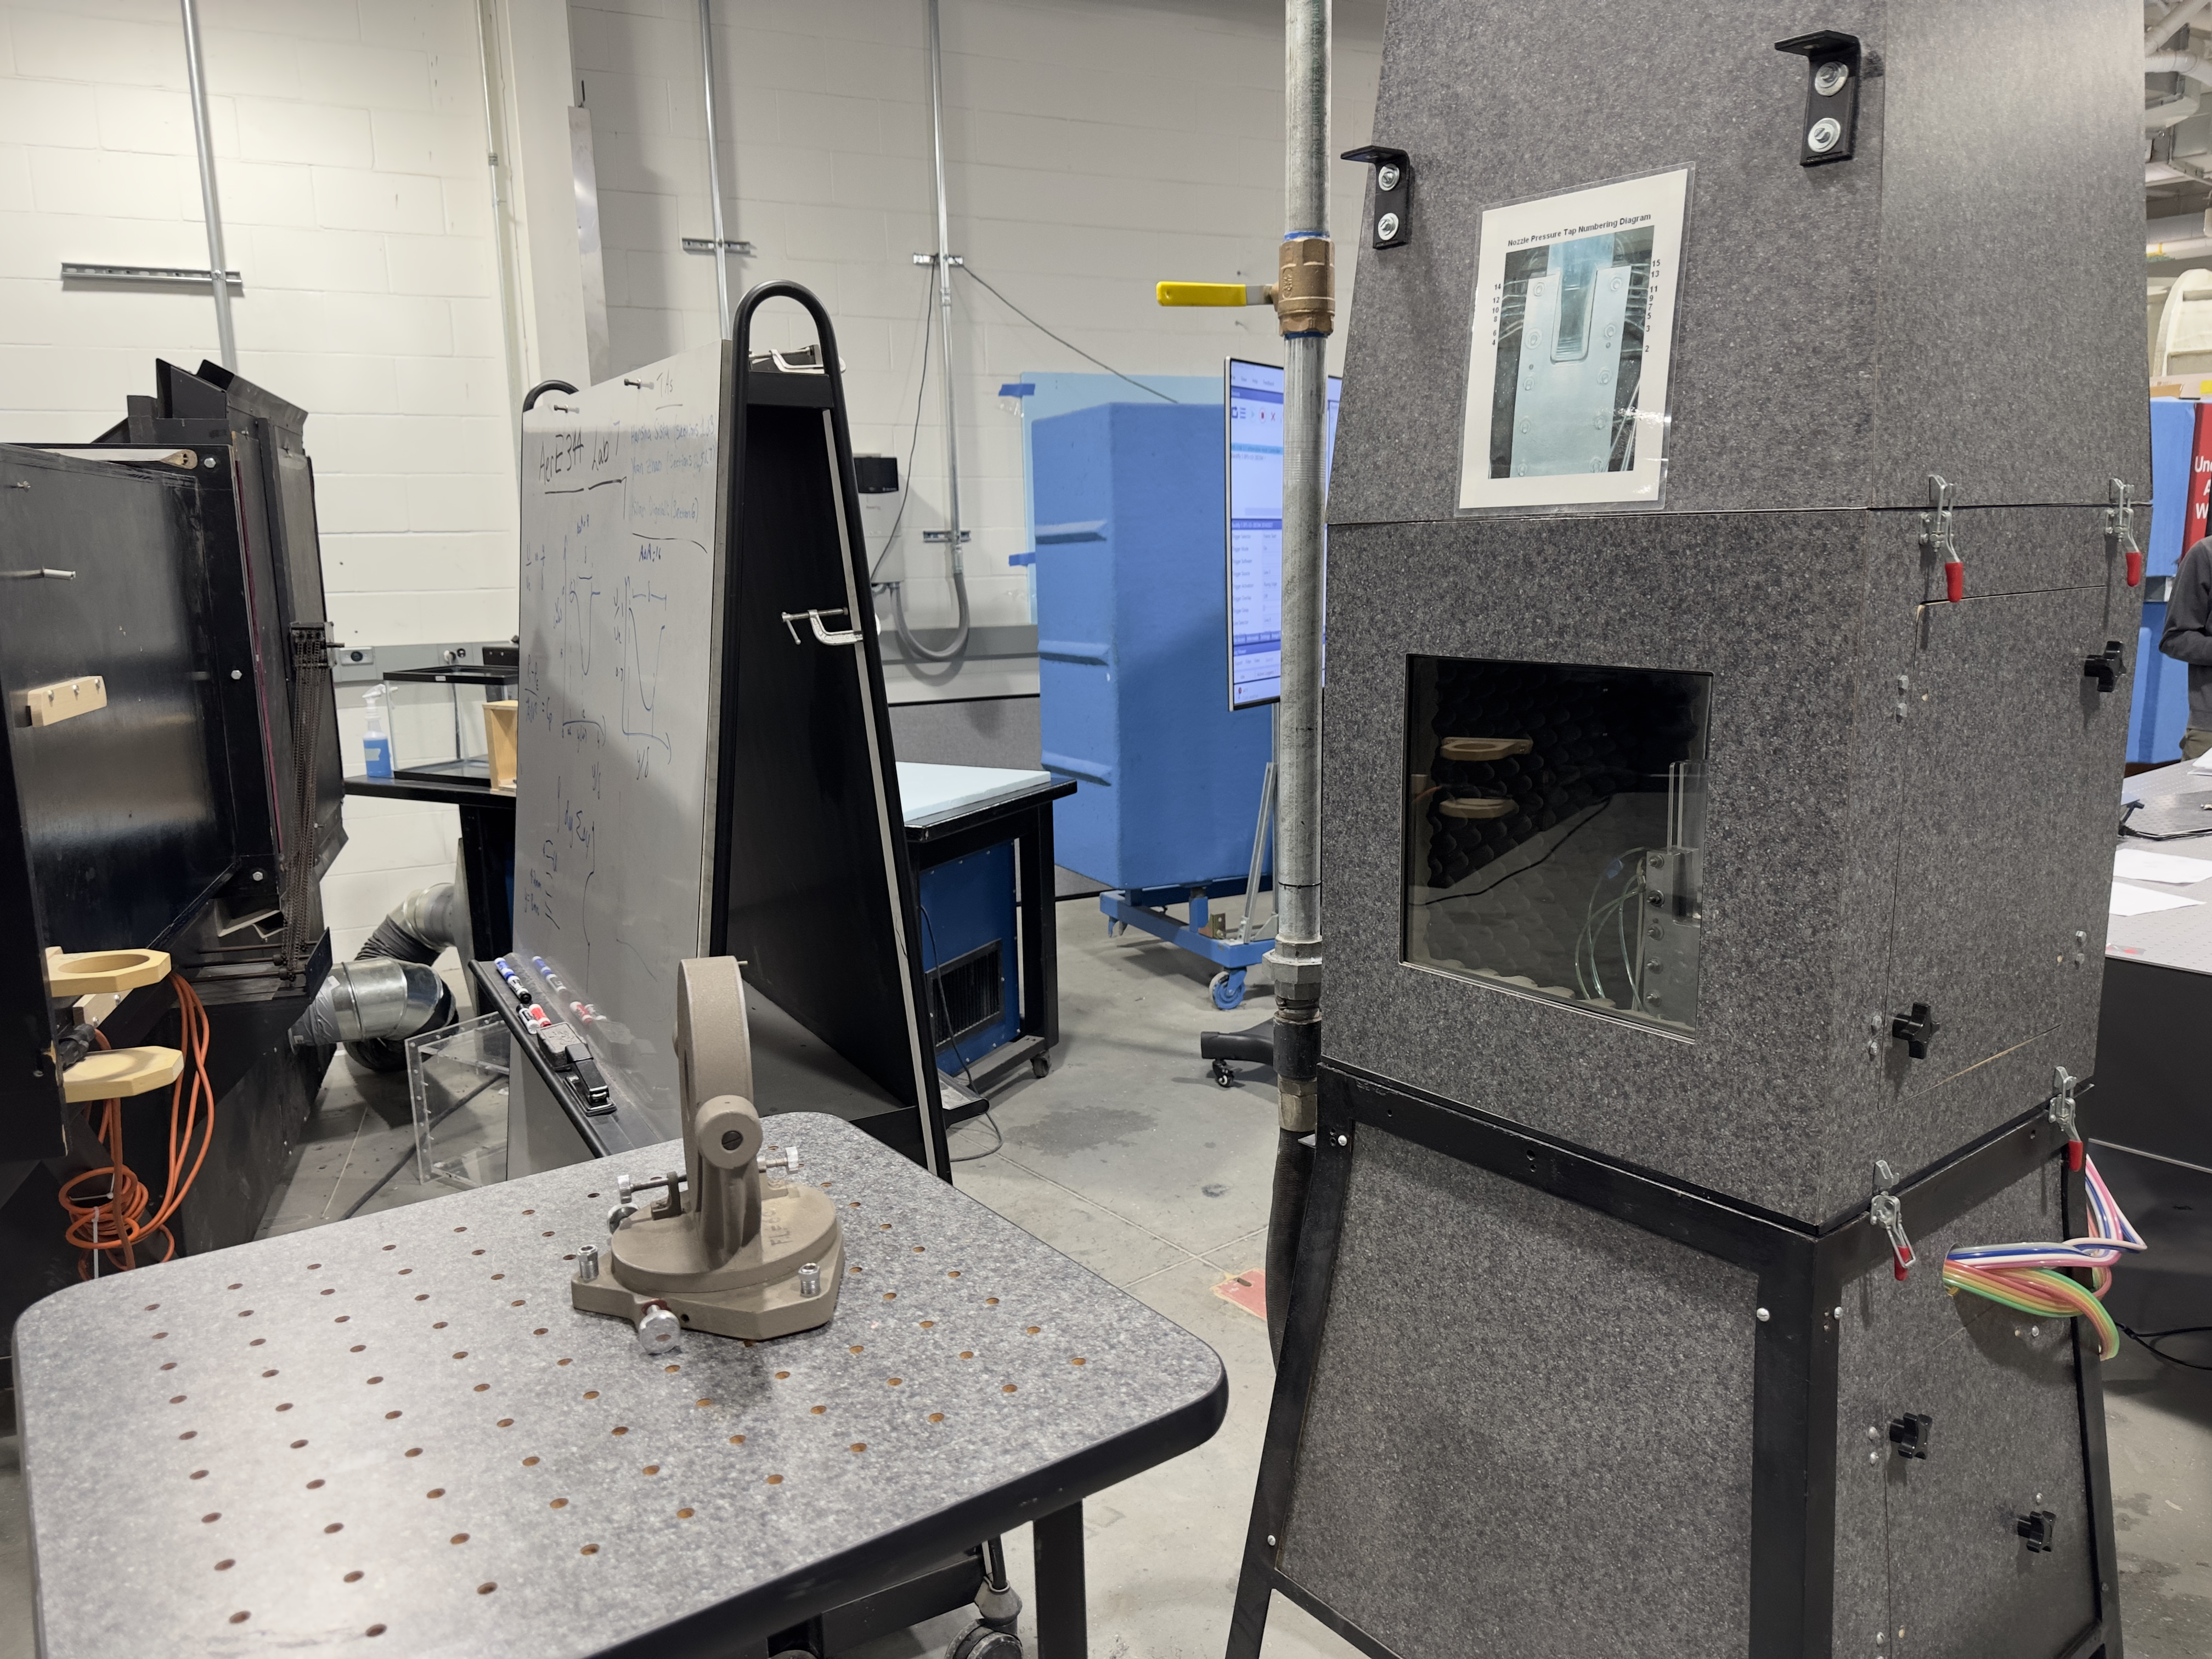
\includegraphics[width=0.75\linewidth]{Figures/back_of_supersonic_wind_tunnel.jpeg}
    \caption{The supersonic wind tunnel.}
    \label{fig:supersonic_wind_tunnel}
\end{figure}

\begin{figure}[htpb]
    \centering
    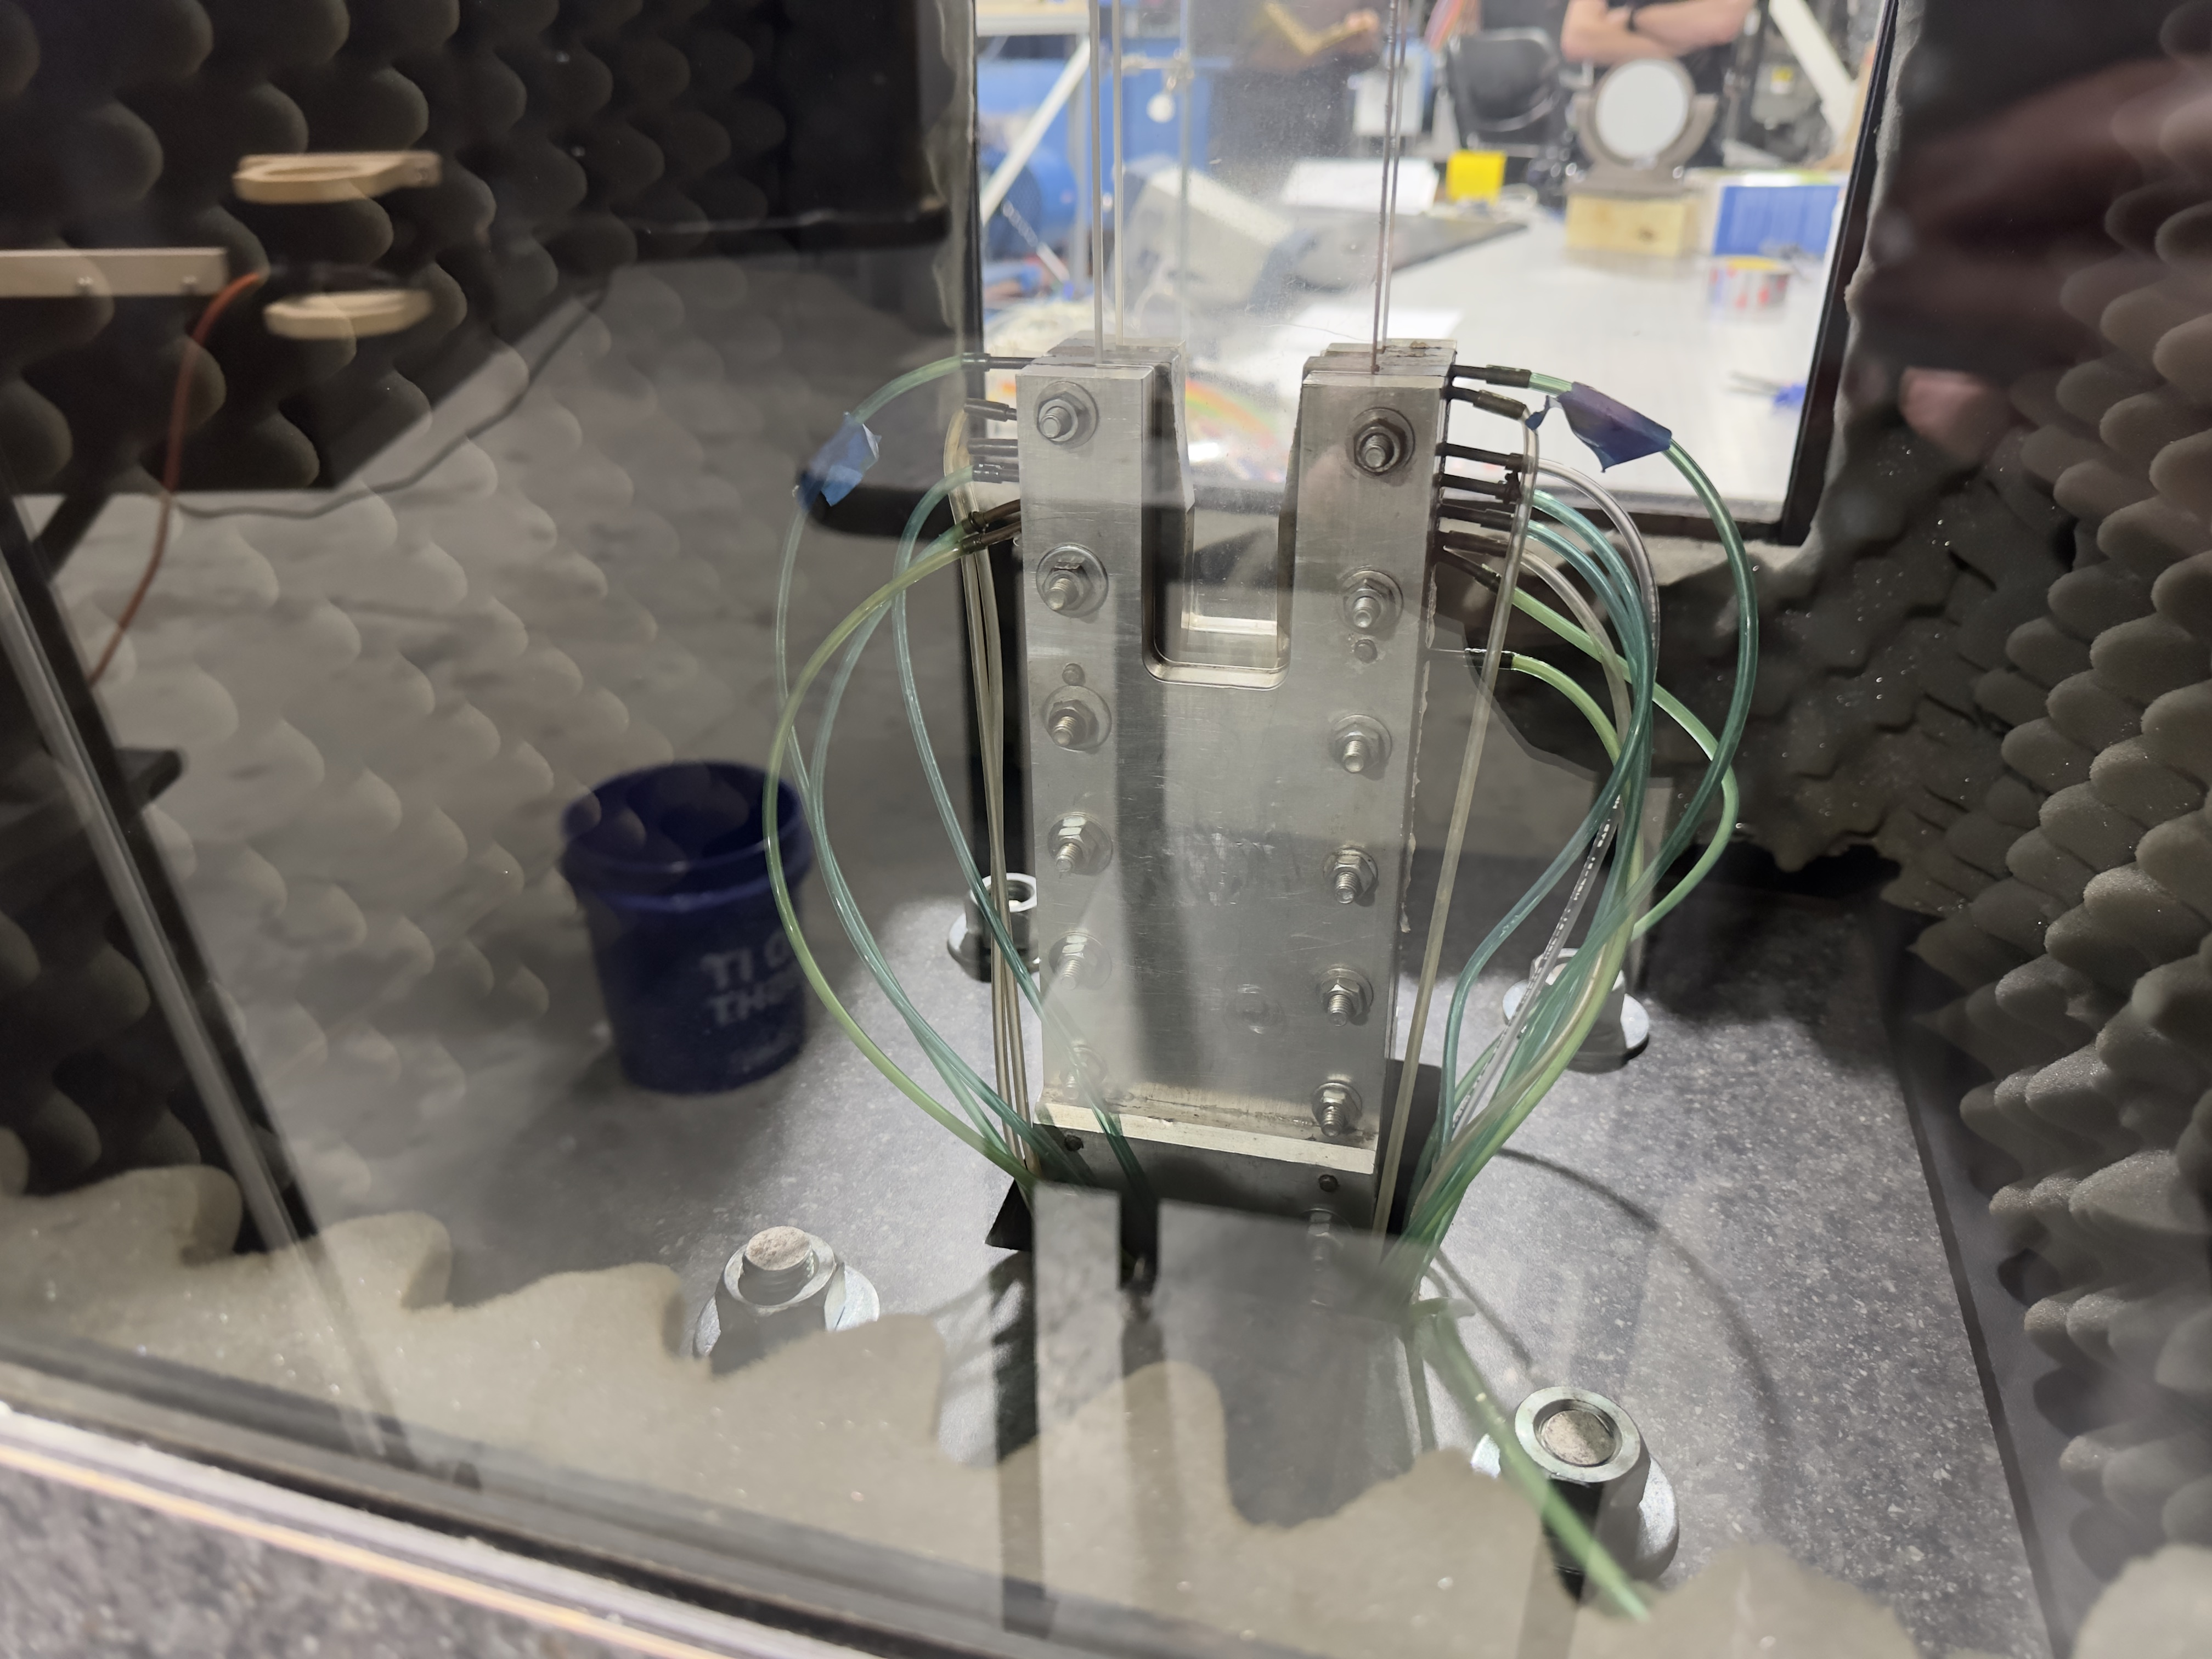
\includegraphics[width=0.75\linewidth]{Figures/de_laval_nozzle.jpeg}
    \caption[The de Laval nozzle in the supersonic wind tunnel.]{The de Laval nozzle in the supersonic wind tunnel. The pressure taps are connected to a pressure transducer which is further connected to the data acquisition computer.}
    \label{fig:de_laval_nozzle}
\end{figure}

\begin{figure}[htpb]
    \centering
    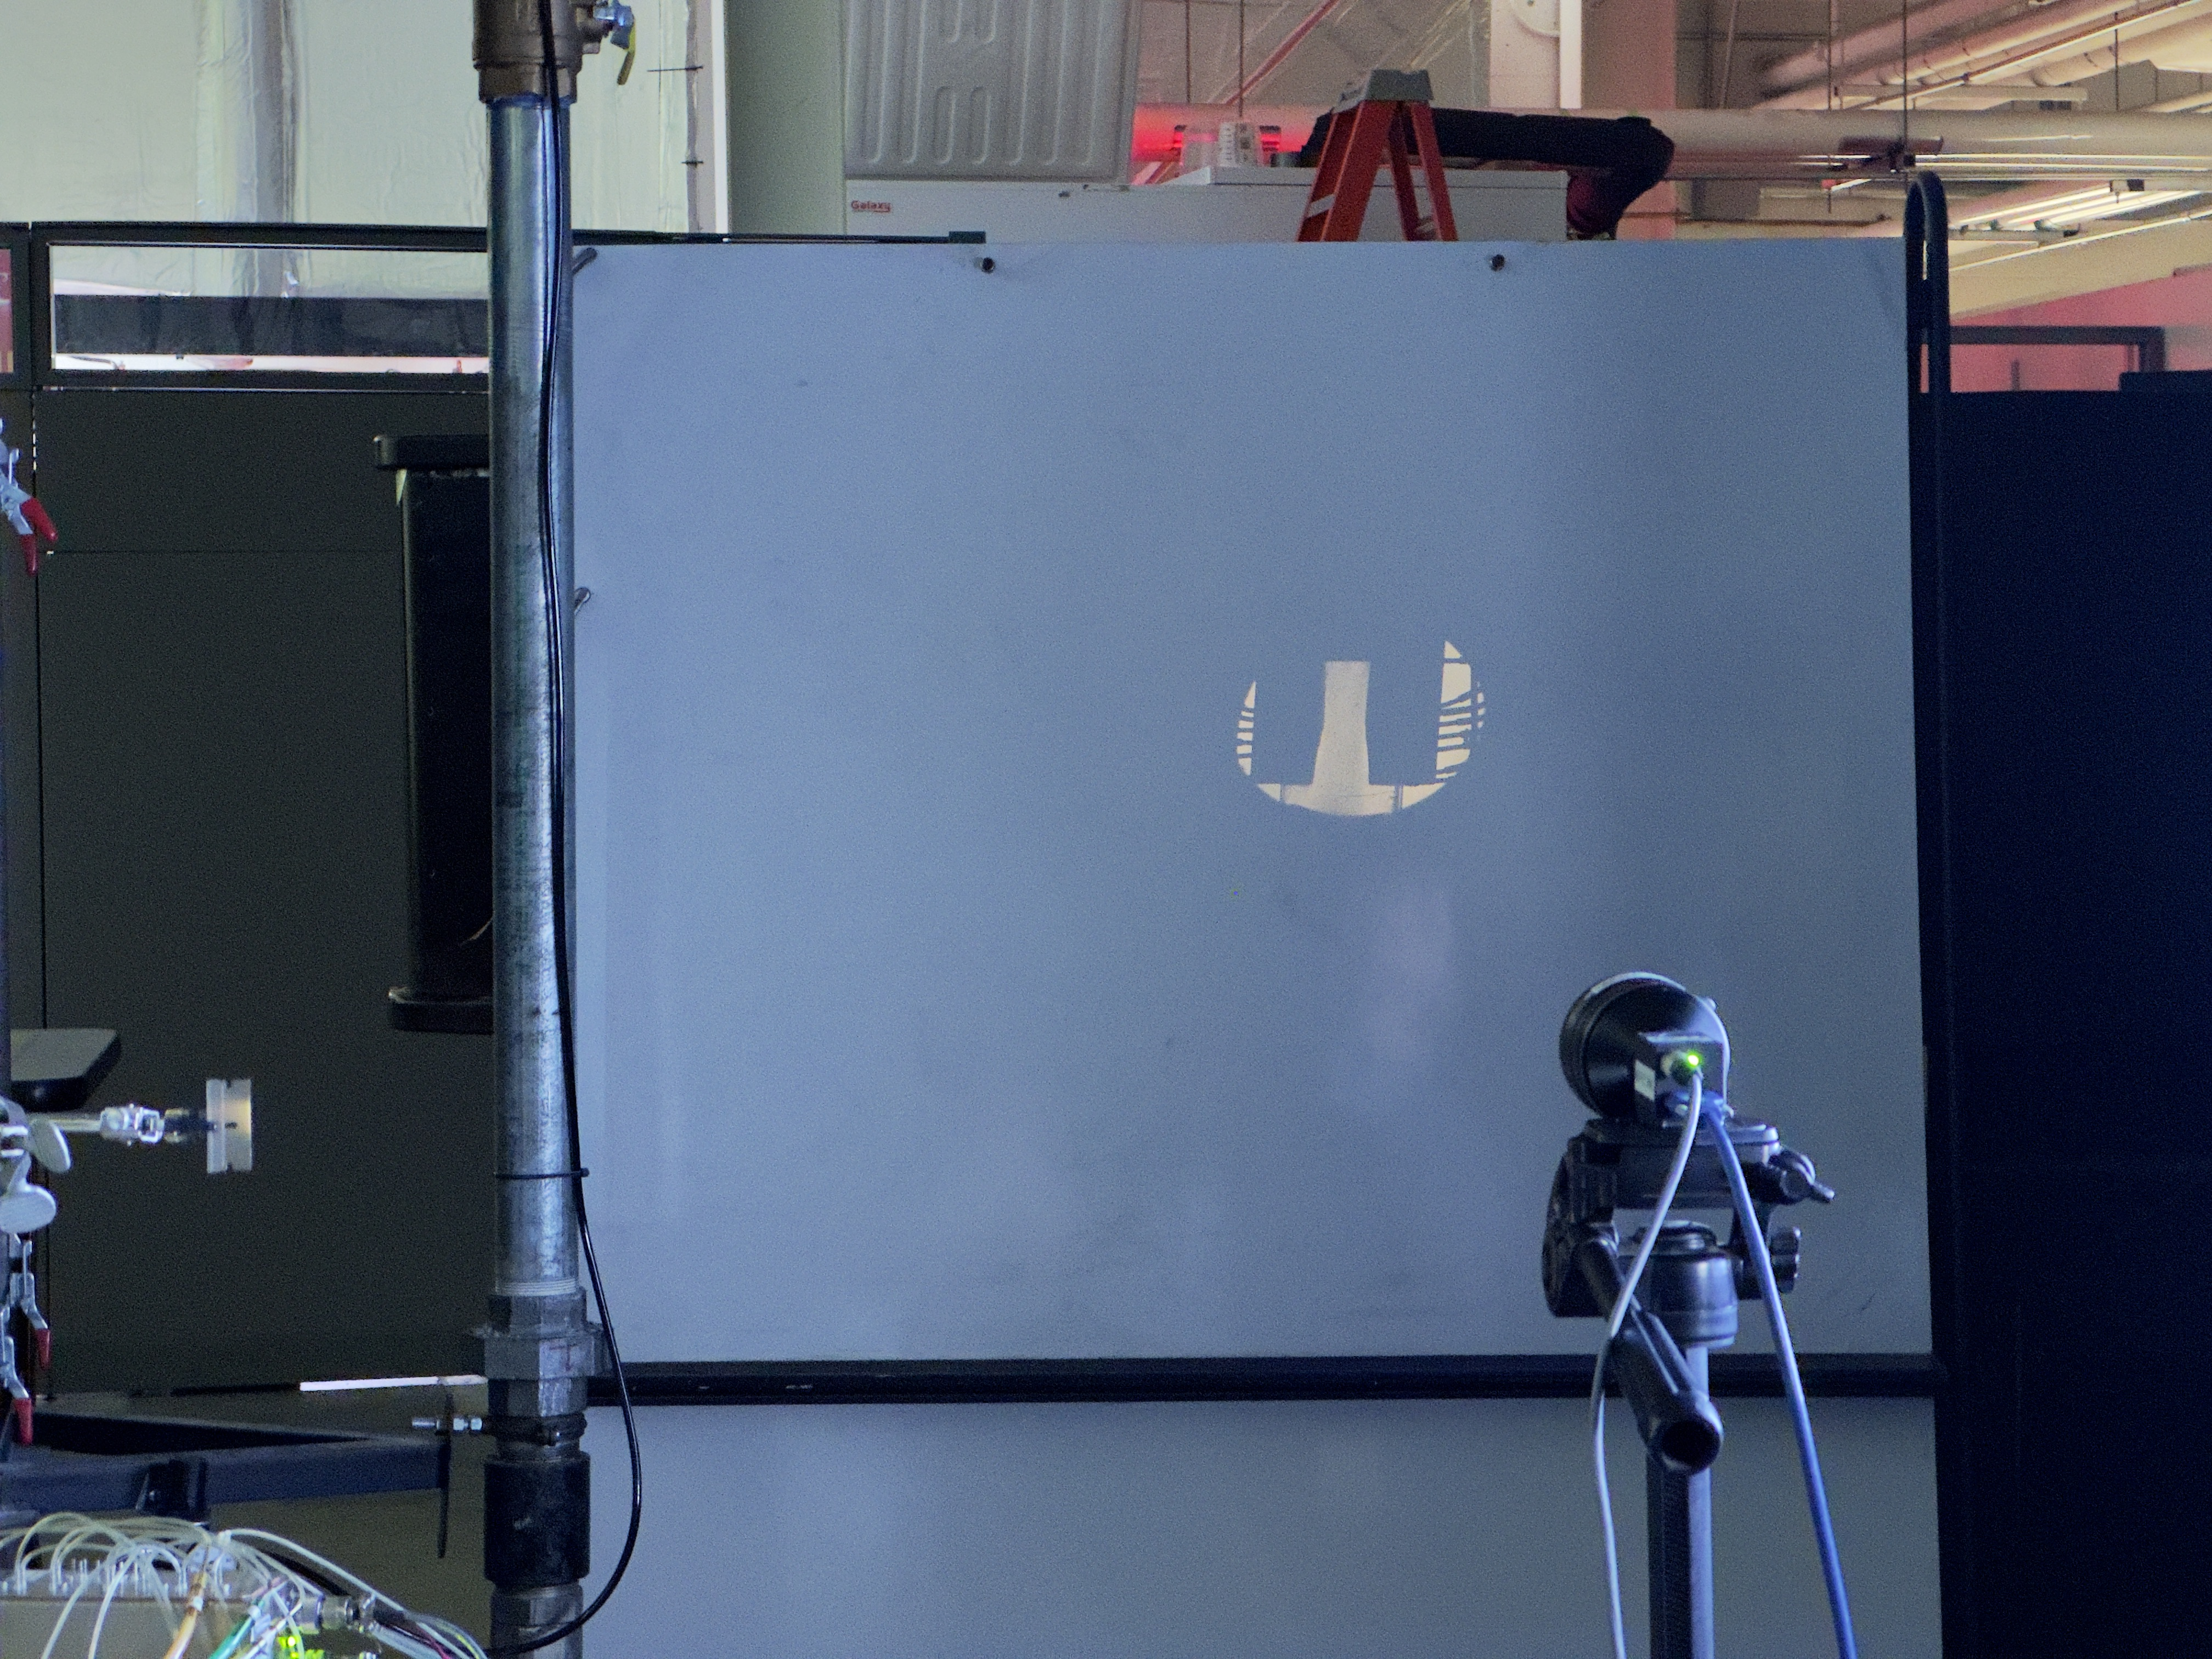
\includegraphics[width=0.75\linewidth]{Figures/schlieren_nozzle.jpeg}
    \caption[A Schlieren projection of the flow moving through the de Laval nozzle being projected onto a white board.]{A Schlieren projection of the flow moving through the de Laval nozzle being projected onto a white board. The camera takes close-up, high-contrast images of the projection.}
    \label{fig:schlieren_projection}
\end{figure}

\section{Procedure} \label{sec:procedure}

\begin{enumerate}
    \item Pressurize the air tank connected to the supersonic wind tunnel.
    \item Set up the imaging system as described in \autoref{sec:apparatus}.
    \item Start recording data using the data collection software and open the valve to release the air into the wind tunnel.
    \item When the tank is empty, close the valve.
\end{enumerate}

\section{Derivations} \label{sec:derivations}

The six states we were directed to note the data positions of are as follows:

\begin{enumerate}
    \item under-expanded flow
    \item third critical condition
    \item over-expanded flow
    \item second critical condition
    \item normal shock inside the divergent section of the nozzle
    \item first critical condition
\end{enumerate}

\noindent{}however, as described in \autoref{sec:theoretical_calculations}, we will only generate plots and comparisons for the third critical condition, second critical condition, normal shock inside the divergent section of the nozzle, and the first critical condition.

There are a number of calculations that must be performed on the measured data before it can be compared to the theoretical calculations. The details of these calculations for the measured and theoretical scenarios can be found in \autoref{sec:measured_calculations} and \autoref{sec:theoretical_calculations}, respectively.

For the sake of comparison, we choose picture or data point number \num{168} (zero-indexed) for our state with a normal shock in the divergent section of nozzle. The image from this data point is shown in \autoref{fig:schlieren_overlay} with the schematic of the de Laval nozzle overlaid. The data shows a significant drop in static pressure between pressure taps \num{10} and \num{11}, but from the image, it appears that the normal shock is in between pressure tap \num{11} and \num{12}.

\begin{figure}[htpb]
    \centering
    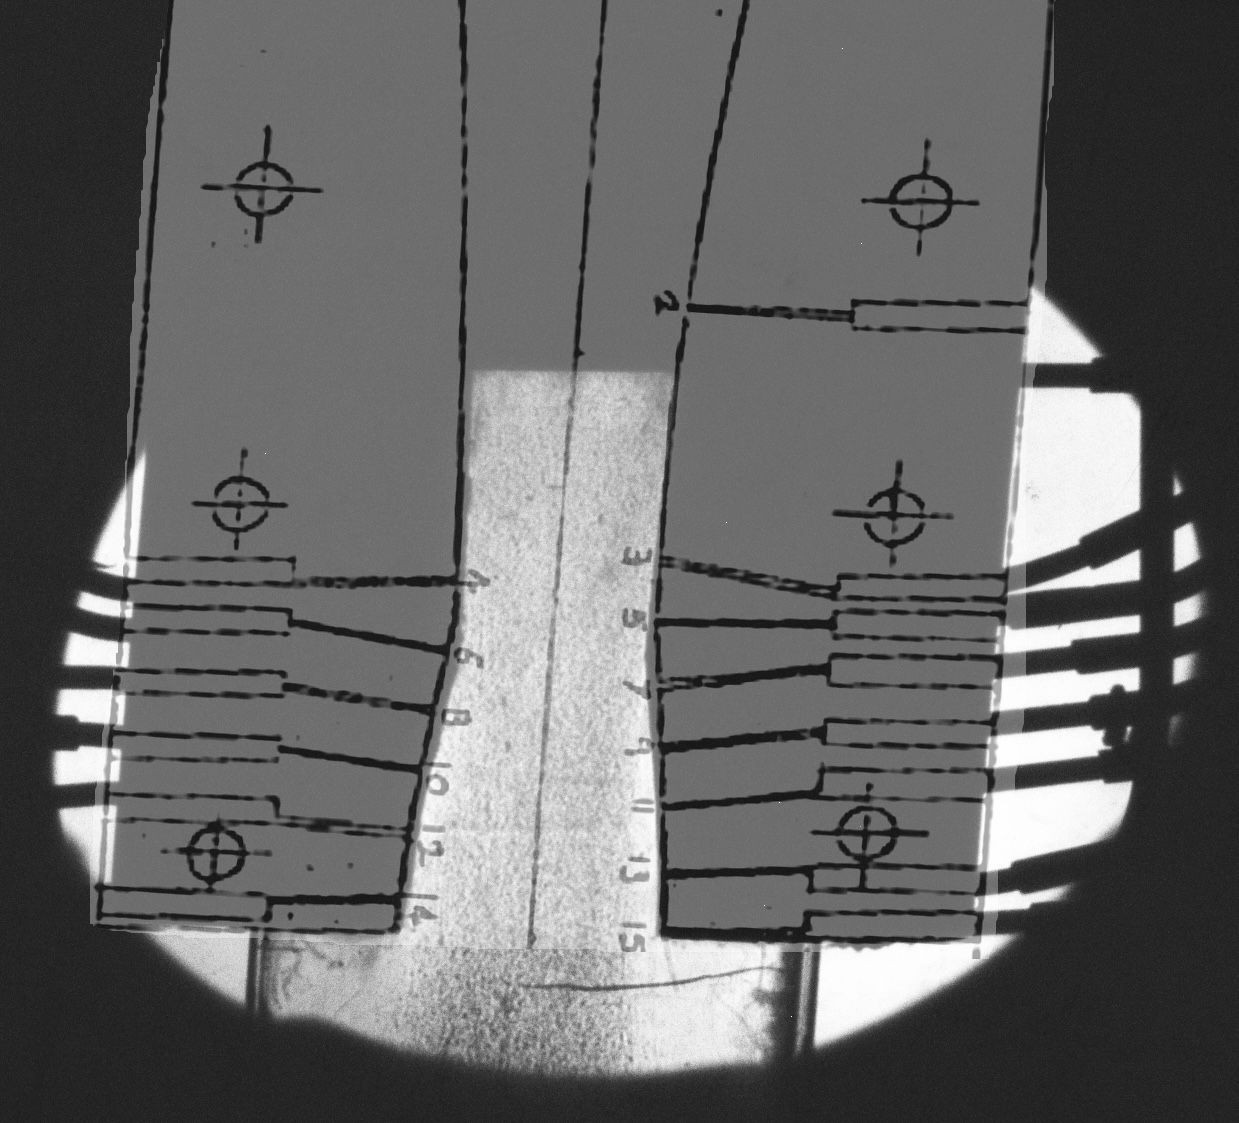
\includegraphics[width=0.75\linewidth]{Figures/Nozzle Overlay with Shock.jpg}
    \caption[An overlay of the de Laval nozzle schematic and an image of the nozzle when a normal shock is present.]{An overlay of the de Laval nozzle schematic and a Schlieren image capture of the de Laval nozzle when the shock is inside the divergent section of the nozzle.}
    \label{fig:schlieren_overlay}
\end{figure}

Because of the boundary layer conditions, the normal shock does not span straight across the nozzle, and the slight curvature of the shock near the edges of the nozzle may explain why the shock appears to be between taps \num{11} and \num{12} but the pressure drop occurs between taps \num{10} and \num{11}. For the sake of analysis, we chose to assume the normal shock occurred between pressure taps \num{10} and \num{11} with the pressure at tap \num{10} and \num{11} denoted \gls{P_1} and \gls{P_2}, respectively.

The data analysis for this lab was performed in \acrfull{matlab} (see \autoref{cp:scripts}).

\subsection{Measured Calculations} \label{sec:measured_calculations}

The general procedure we followed for the measured pressure and mach number calculations is described generally in \citet{lab10-manual}. The first step is to convert the pressure tap data from gauge pressure to absolute pressure which is accomplished with \autoref{eqn:absolute_pressure_eqn}.

\begin{equation} \label{eqn:absolute_pressure_eqn}
    P = P_g + P_\text{atm}
\end{equation}

\noindent{}\gls{P} is static pressure, \gls{P_g} is the gauge pressure measurement, and \gls{P_atm} is atmospheric pressure, which we were given as $P_\text{atm} = \qty{1010}{\milli\bar}$.

Once the pressure data is converted to absolute pressure, we solve for the total pressure of each state by assuming the flow was choked at the throat—\textit{i.e.}, the Mach number at the throat is \num{1}—and plugging the measured static pressure values at the throat into the total-static relation, \autoref{eqn:total-static_relation}.

\begin{equation} \label{eqn:total-static_relation}
    \frac{P_0}{P} = \left(1 + \frac{\gamma - 1}{2}M^2\right)^\frac{\gamma}{\gamma - 1}
\end{equation}

\noindent{}\gls{P_0} is the total pressure, \gls{P} is the static pressure, \gls{gamma} is the ratio of specific heats for air (defined as \num{1.4} for air), and \gls{M} is the Mach number. This correctly calculates the total pressure throughout the nozzle for each of the states, except for the state in which a normal shock is present in the nozzle. Since total pressure drops across a normal shock, it is necessary to re-calculate the total pressure after the normal shock using normal shock formulas.

To correct the total pressure for the normal shock state, we first must find the Mach number before the shock. To calculate the measured Mach number throughout the nozzle for each of the states, we again use the total-static relation, \autoref{eqn:total-static_relation}. Instead of solving for total pressure with a known Mach number, we solve \autoref{eqn:total-static_relation} for the Mach number by using the measured total pressures calculated above and the measured static pressure values from the pressure taps. Similar to the total pressure calculation, this Mach distribution is valid for all the states except for the state with a normal shock in the nozzle.

Now armed with the total pressure and Mach number before the shock, we correct the total pressure and then the Mach number after the shock for the state where there is a normal shock in the nozzle. Let \gls{M_1} be the Mach number immediately before the shock (tap \num{10})—which we calculated when we calculated the Mach distribution above—and \gls{M_2} be the Mach number immediately after the shock (tap \num{11}). Then, we use \autoref{eqn:normal_shock_eqn} to calculate \gls{M_2}.

\begin{equation} \label{eqn:normal_shock_eqn}
    M_2 = \sqrt{\frac{1 + \frac{\gamma - 1}{2}M_1^2}{\gamma M_1^2 - \frac{\gamma - 1}{2}}}
\end{equation}

Once we have \gls{M_2}, which is the estimated Mach number immediately after the shock, we use that Mach number with the measured static pressure at tap \num{11} to find the estimated total pressure after the shock by, once more, evaluating the total-static relationship, \autoref{eqn:total-static_relation}.

Now that the total pressure downstream of the shock is correct for the normal shock state, we recalculate the Mach distribution downstream of the normal shock. It should come as no surprise that this is accomplished using \autoref{eqn:total-static_relation}.

\subsection{Theoretical Calculations} \label{sec:theoretical_calculations}

Although we identified six different states from the Schlieren imagery (see \autoref{fig:schlieren_projection}), only four of the states have trivial theoretical solutions, namely:

\begin{itemize}
    \item first critical condition
    \item normal shock in the nozzle
    \item second critical condition
    \item third critical condition
\end{itemize}

\noindent{} the other two states, over-expanded and under-expanded flow, would require assumptions about the the nature of the oblique and expansion shocks occurring at the exit of the nozzle. Hence, while all the calculations we performed in \autoref{sec:measured_calculations} were valid for each of the six states, in this section, we will only consider the four states listed above.

This first step in the theoretical calculations is to calculate a Mach distribution for each of the states. We start by assuming each of the states is choked, subsonic before the throat, supersonic after the throat, and that there are no shocks in the nozzle. For the appropriate states, we will correct these invalid assumptions later. If these assumptions are all true, calculating the mach distribution is as trivial as evaluating the Mach number in \autoref{eqn:AbyAstar} using \verb|fsolve()|.

\begin{equation} \label{eqn:AbyAstar}
    \frac{A}{A^*} = \frac{\left(5 + M^2\right)^3}{6^3M}
\end{equation}

\noindent{}\gls{A} is the area at a particular pressure tap, \gls{Astar} is the area of the sonic throat, and \gls{M} is the Mach number at the corresponding pressure tap \citep{2024durbin}. The area measurements were provided in units of \unit{in^2} by the lab manual \citep{lab10-manual}.

For the first critical condition, the flow is subsonic before \textit{and} after the throat—as opposed to subsonic before and supersonic after. To correct the Mach distribution after the throat, we use \autoref{eqn:AbyAstar} again and change the initial condition of \verb|fsolve()| to calculate the subsonic Mach solution.

In the state where there is a normal shock in the divergent section of the de Laval nozzle, we must fix the Mach distribution downstream of the normal shock. The process is similar to the one described in \autoref{sec:measured_calculations}. First, we determine \gls{M_1}—the theoretical Mach number at tap \num{10}—and then calculate \gls{M_2}—the theoretical Mach number downstream of the normal shock at tap \num{11}—using \autoref{eqn:normal_shock_eqn}. Then, with \gls{M_2} and the area immediately downstream of the shock, we use \autoref{eqn:AbyAstar} to evaluate \gls{Astar2}, the virtual or reference sonic throat area downstream of the normal shock. Using \gls{Astar2}, we then correct the Mach distribution downstream of the normal shock with \autoref{eqn:AbyAstar} (using a subsonic initial value for \verb|fsolve()|).

With the Mach distribution squared away, we turn our attention to the theoretical pressure distributions. For the first critical condition, the normal shock in the nozzle, and the third critical condition, the pressure at the exit of the nozzle is, by definition, equivalent to the ambient pressure, \gls{P_atm}. Using \autoref{eqn:total-static_relation}, we can find the total pressure for each of the states.

Just as in the other calculations, for the state where there is a normal shock in the nozzle, the total pressure value we just calculated will be invalid for the flow upstream of the normal shock. To determine the proper theoretical total pressure upstream of the shock, we utilize a useful fact about normal shocks in de Laval nozzles:

\begin{equation} \label{eqn:shock_in_nozzle}
    P_{01}A_1^* = P_{02}A_2^*
\end{equation}

\noindent{}where \gls{P_01} and \gls{Astar1} is the total pressure and sonic throat area upstream of the shock and \gls{P_02} and \gls{Astar2} is the total pressure and sonic throat area downstream of the shock. Since we are given \gls{Astar1}, we calculated \gls{Astar2} when we calculated the theoretical Mach distribution downstream of the normal shock, and we calculated \gls{P_02} when we evaluated the total pressure downstream of the normal shock based on the ambient exit pressure, calculating \gls{P_01} is trivial.

To determine the total pressure when the flow is in the second critical condition, we must be slightly more clever. By definition, the second critical condition occurs when there is a normal shock \textit{exactly} at the exit of the nozzle. Since the flow downstream of a normal shock must be subsonic, we know the pressure immediately after the normal shock is equivalent to the ambient pressure. Additionally, since we know the Mach number at the exit of the nozzle from our Mach distribution calculations above, we use the normal shock relationship in \autoref{eqn:normal_shock_pressure_eqn} to determine the static pressure at the exit of the nozzle—prior to the normal shock.

\begin{equation} \label{eqn:normal_shock_pressure_eqn}
    \frac{P_2}{P_1} = \frac{7M_1^2 - 1}{6}
\end{equation}

\noindent{}\gls{P_1} is the static pressure upstream of the shock, \gls{P_2} is the static pressure downstream of the shock, and \gls{M_1} is the Mach number immediately upstream of the normal shock.

Now that we know the static pressure at the exit of the nozzle just prior to the normal shock, we can use our favorite \autoref{eqn:total-static_relation} to find the total pressure throughout the nozzle. Since the flow in the nozzle prior to the normal shock is isentropic in the second critical condition, this is the total pressure for the entire nozzle.

Finally, to find the theoretical pressure distribution, we plug our theoretical total pressure distribution and our theoretical Mach number distribution into the wonderful \autoref{eqn:total-static_relation}.

Our \acrshort{matlab} script automatically extracts the data file, performs these calculations, plots the data, saves the plots to \verb|.svg| files, prints the tables in \autoref{sec:data_tables} to \verb|.tex| files, and deletes the extracted data file.